\subsection{Recurrent Neutral Networks}
\label{RNN}
Recurrent Neutral Networks (RNN) sind eine spezielle Form des künstlichen neuronalen Netzes, die besonders für die Verarbeitung von Sequenzen (z.B. Zeitreihen oder Wortvorhersagen) geeignet sind.\\

\textbf{One-Hot-Kodierung}: Vektorierung von Kategorien, sodass jede Kategorie durch einen Vektor repräsentiert wird, der nur eine $1$ an der Stelle der Kategorie hat, sonst $0$, z.B.
\begin{equation*}
    \begin{aligned}
        \text{Kategorien: } &\text{Apfel, Banane, Birne}\\
        \text{One-Hot-Kodierung: } &\text{Apfel} = \begin{pmatrix}
            1\\
            0\\
            0
        \end{pmatrix}, \text{Banane} = \begin{pmatrix}
            0\\
            1\\
            0
        \end{pmatrix}, \text{Birne} = \begin{pmatrix}
            0\\
            0\\
            1
        \end{pmatrix}
    \end{aligned}
\end{equation*}

\underline{\textbf{Eigenschaften}}:
\begin{itemize}
    \item Kategorien/Vokabular ist vollständig definiert $\rightarrow$ feste Anzahl an Kategorien
    \item Anzahl an Eingaben (z.B. Wörter) kann variieren $\rightarrow$ anders als Feedforward-Netzwerke mit fixer Anzahl
    \item Wie bei CNN: Lokalität und Paramter Sharing, spätere Vorhersagen werden konzeptionell so behandelt, wie frühere Vorhersagen\\
\end{itemize}

\underline{\textbf{Aufbau}}:

\begin{figure}[H]
    \centering
    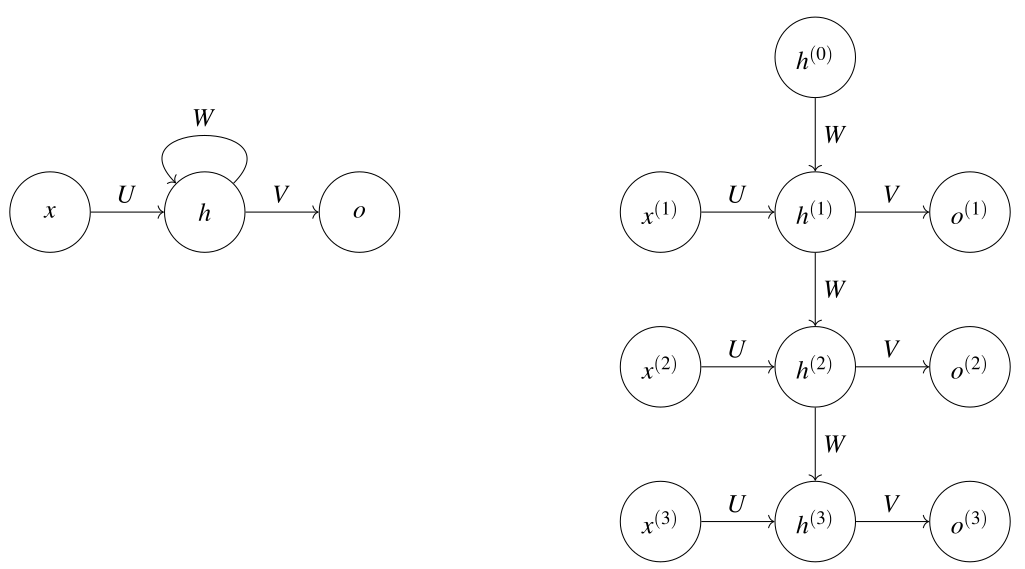
\includegraphics[width=0.5\textwidth]{deepLearning/rnn_overview.png}
    \caption{Übersicht eines RNN}
\end{figure}
Beginnend bei einem initialen Zustand $h^{(0)}$ wird für jede Eingabe $x^{(i)}$ mittels Parametermatrix $U$ ein neuer (\emph{hidden}) Zustandsvektor $h^{(i)}$ berechnet. Dieser Vektor wird zum einen zur Bestimmung einer (Zwischen-)Ausgabe $o^{(i)}$ (mittels Gewichtsmatrix $V$) und zum anderen zur Bestimmung eines neuen (versteckten) Zustands $h^{(i+1)}$ (mittels Gewichtsmatrix $W$ und Aktivierungsfunktion $\text{act()}$) verwendet. $h$ fungiert hierbei als eine Art \emph{Gedächtinis}:\\

\begin{equation*}
    \begin{aligned}
        h^{(i)} &= \text{act}(Ux^{(i)} + Wh^{(i-1)})\\
        o^{(i)} &= \text{act}(Vh^{(i)})
    \end{aligned}
\end{equation*}

\underline{\textbf{Probleme}}:
\begin{itemize}
    \item \emph{Vanishing Gradient}: Gradienten werden bei der Rückwärtspropagierung durch Wiederholte Multiplikation mit $W$ so klein, dass sie kaum noch Einfluss auf die Gewichtsanpassung haben.
    \item \emph{Long-Term Dependencies}: RNNs haben Schwierigkeiten, lange Abhängigkeiten zu lernen, da der Gradient bei der Rückwärtspropagierung durch viele Schichten hindurchgehen muss (s.o. wdh. Multipl. mit $W$).
\end{itemize}
Lösung der Probleme zB. über LSTM (Long Short-Term Memory; spezielle RNN-Architektur).\\